% VDE Template for EUSAR Papers
% Provided by Barbara Lang und Siegmar Lampe
% University of Bremen, January 2002
% English version by Jens Fischer
% German Aerospace Center (DLR), December 2005
% Additional modifications by Matthias Wei{\ss}
% FGAN, January 2009

%-----------------------------------------------------------------------------
% Type of publication
\documentclass[a4paper,10pt]{article}
%-----------------------------------------------------------------------------
% Other packets: Most packets may be downloaded from www.dante.de and
% "tcilatex.tex" can be found at (December 2005):
% http://www.mackichan.com/techtalk/v30/UsingFloat.htm
% Not all packets are necessarily needed:
\usepackage[T1]{fontenc}
\usepackage[latin1]{inputenc}
%\usepackage{ngerman} % in german language if required
\usepackage[nooneline,bf]{caption} % Figure descriptions from left margin
\usepackage{times}
\usepackage{multicol}
\usepackage{amsmath}
\usepackage{amssymb}
\usepackage{graphicx}
\usepackage{epsfig}
\input{tcilatex}
%-----------------------------------------------------------------------------
% Page Setup
\textheight24cm \textwidth17cm \columnsep6mm
\oddsidemargin-5mm                 % depending on print drivers!
\evensidemargin-5mm                % required margin size: 2cm
\headheight0cm \headsep0cm \topmargin0cm \parindent0cm
\pagestyle{empty}                  % delete footer and header
%----------------------------------------------------------------------------
% Environment definitions
\newenvironment*{mytitle}{\begin{LARGE}\bf}{\end{LARGE}\\}%
\newenvironment*{mysubtitle}{\bf}{\\[1.5ex]}%
\newenvironment*{myabstract}{\begin{Large}\bf}{\end{Large}\\[2.5ex]}%
%-----------------------------------------------------------------------------
% Using Pictures and tables:
% - Instead "table" write "tablehere" without parameters
% - Instead "figure" write "figurehere " without parameters
% - Please insert a blank line before and after \begin{figuerhere} ... \end{figurehere}
%
% CAUTION:   The first reference to a figure/table in the text should be formatted fat.
%
\makeatletter
\newenvironment{tablehere}{\def\@captype{table}}{}
\newenvironment{figurehere}{\def\@captype{figure}\vspace{2ex}}{\vspace{2ex}}
\makeatother



%%%%%%%%%%%%%%%%%%%%%%%%%%%%%%%%%%%%%%%%%%%%%%%%%%%%%%%%%%%%%%%%%%%%%%%%%%%%%%
\begin{document}

% Please use capital letters in the beginning of important words as for example
\begin{mytitle}A survey on resource management policies for NUMA architectures\end{mytitle}
%
% Please do not insert a line here
%
\\
Ferrini Francesco\\
Matr. 755508, (goffredoam84@gmail.com)\\
\hspace{10ex}
Gallo Francesco\\
Matr. 755748, (loshura@hotmail.it)\\
\begin{flushright}
\emph{Report for the master course of Embedded Systems}\\
\emph{Reviser: PhD. Patrick Bellasi (bellasi@elet.polimi.it)}
\end{flushright}

Received: April, 01 2011\\
\hspace{10ex}

\begin{myabstract} Abstract \end{myabstract}
abstract

\vspace{4ex}	% Please do not remove or reduce this space here.
\begin{multicols}{2}

%%%%%%%%%%%%%%%%%%%%%%%%%%%%%%%%%%%%%%%%%%%%%%%%%%%%%%%%%%%%%%%%%%%%%%%%%%%%%
\section{Introduction}

Numa (Non-Uniform Access Memory) refers to a computer memory design choice used in multiprocessing, where the memory access time depends on the memory location relative to a processor; in fact NUMA means that it will take longer to access some regions of memory than others.

\begin{figurehere}
 \centering
 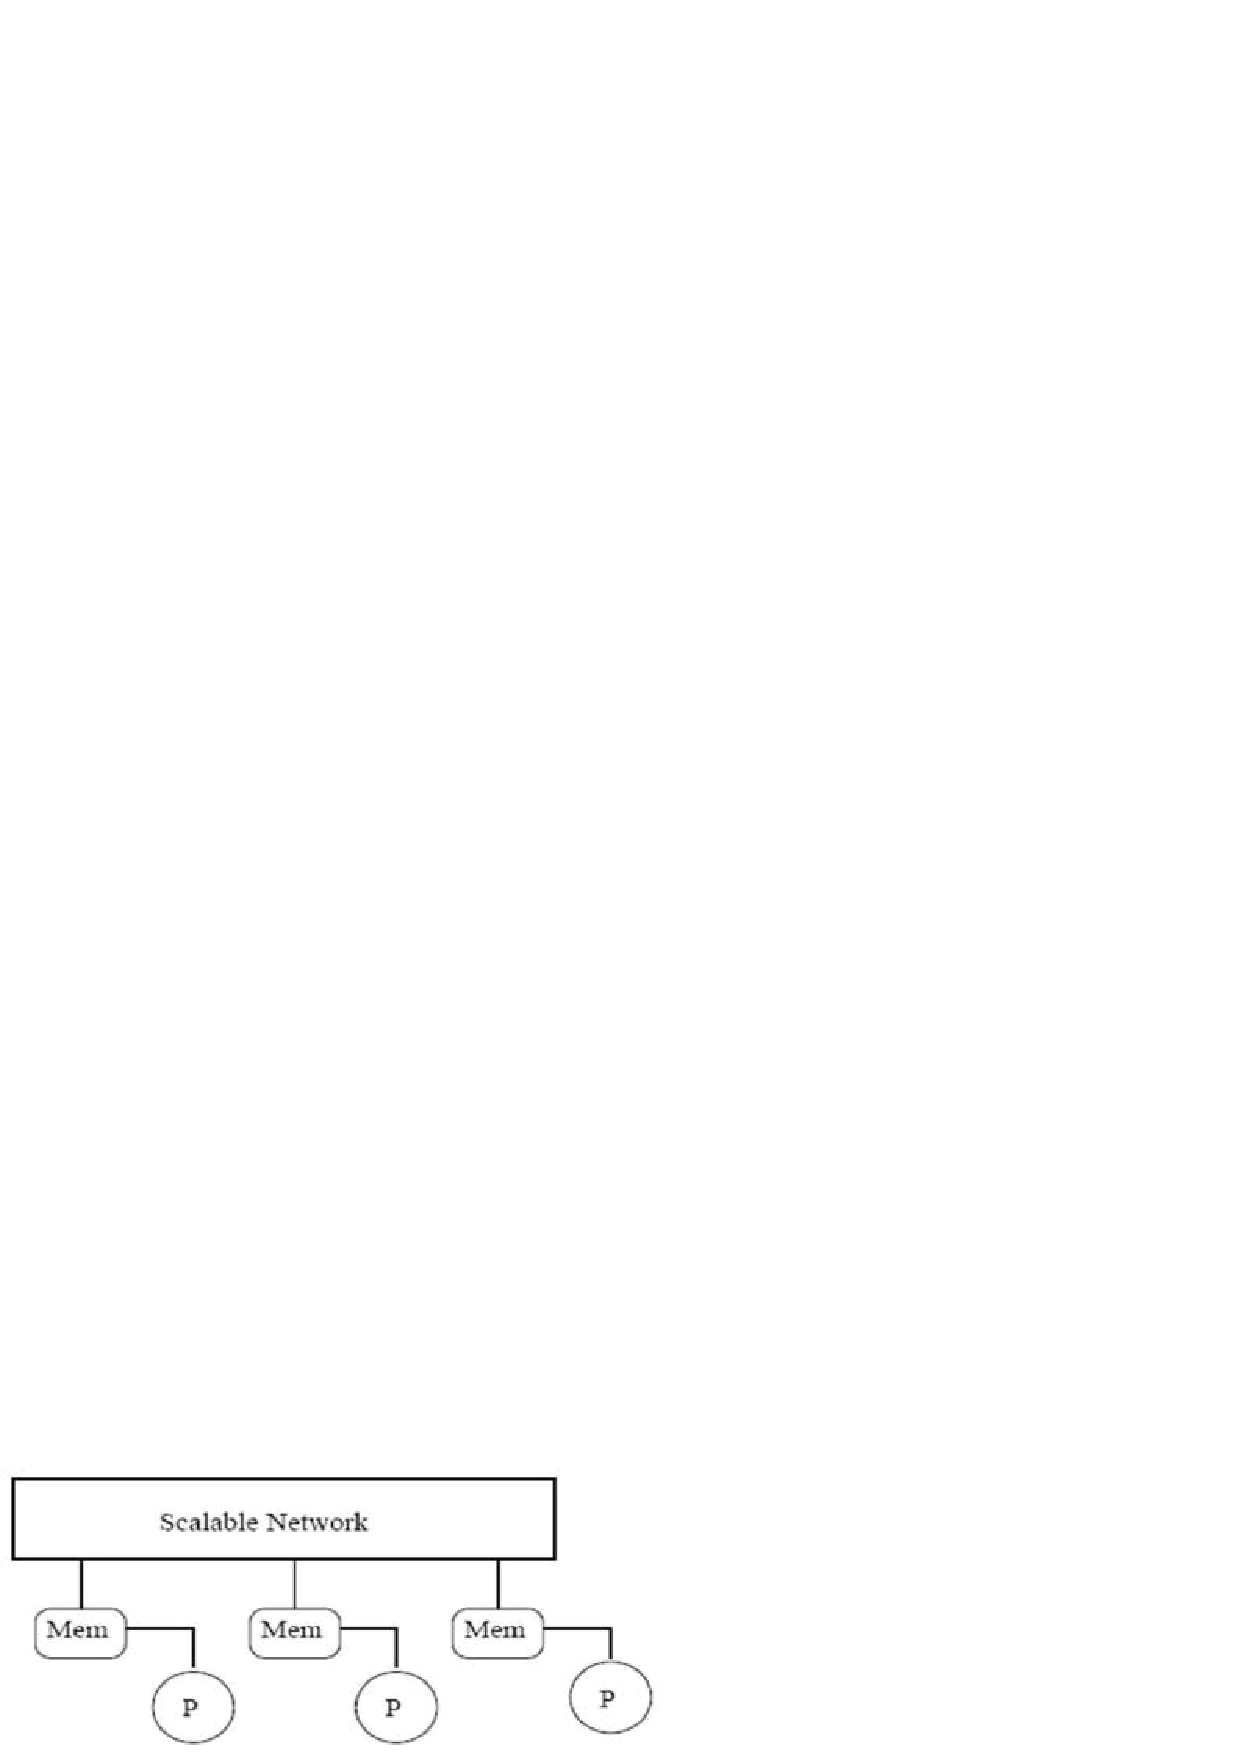
\includegraphics[width=8cm, height=4cm]{./eps/numa.jpg}
 \caption{a simple NUMA architecture design}
 \label{fig:numa}
\end{figurehere}

In Figure \ref{fig:numa} it's possible to see that in a NUMA multiprocessor the physical memory of the system is distributed among individual processors but is still globally addressable by all processors. Sometimes, it is preferable to have more than one processor in the same area. Each of this computational area containing memory block and CPU, whether it has one or more processors, is called node.Thus the cost of a memory access is dependent on where the memory unit addressed is located; relative to the processor some accesses may be local some may be remote. So, with the introduction of NUMA, data locality becomes an important factor because memory accesses have different costs depending on which memory unit is addressed. The scheduling module in the OS must cooperate with the memory management in order to let an application access data mostly from the local memory. NUMA systems can be classified in two categories, both for memory and for processor; regarding memory there are symmetrical and asymmetrical distribution, meaning that accessing different memory nodes can or cannot cost the same. Concerning processor it is possible to have homogeneous system, meaning that all processors are equal in speed and processing power, opposed to heterogeneous ones, where processors have different specifications even inside the same node. This type of architecture turns out to be exposed to some problems, and the most important are: cache coherence, scheduling and memory management.\par
\parindent 10mm In multiprocessor systems it is important to ensure cache coherency. If each processor has a cache that reflects the state of various parts of memory, it is possible that two or more caches may have copies of the same line. It is also possible that a given line may contain more than one lockable data item. If two threads make appropriately serialized changes to those data items, the result could be that both caches end up with different, incorrect versions of the line of memory. In other words, the system's state is no longer coherent because the system contains two different versions of what is supposed to be the content of a specific area of memory. There are 2 types of NUMA architectures that we have to analyse: NCC-NUMA (Non Cache Coherent) and CC-NUMA (Cache Coherent). In NCC-NUMA systems we have some software solutions, while in CC-NUMA we have a cooperation of both software and hardware solutions.\par 
\parindent 10mmScheduling and memory management are strictly connected; in fact they are used to select the best way to load processes, according to the chosen policy, and decide where to allocate memory concerning that process. The last one is used to decide when it is suitable to migrate a thread from a processor to another one or to a different node; this has an additional cost, due to the migration of the memory associated with the thread. (FIXME....RIVEDERE ULTIMO PARAGRAFO)


%%%%%%%%%%%%%%%%%%%%%%%%%%%%%%%%%%%%%%%%%%%%%%%%%%%%%%%%%%%%%%%%%%%%%%%%%%%%%
\section{Solutions and Methods}

In this chapter will be presented some solutions about the problems introduced in previous section, divided by argument. Evaluations will be considered in the next chapter.

%-----------------------------------------------------------------------------
\subsection{Cache Coherence \\ Section}

As seen before, there are 2 types of NUMA architectures that will be analysed: NCC-NUMA (Non Cache Coherent - NUMA) and CC-NUMA (Cache Coherent - NUMA). \\
\subsubsection{Cache coherence in NCC-NUMA}
In NCC-NUMA systems, [CIT. Software Cache Coherence for Large Scale Multiprocessor - Leonidas I. Kontothanassis and Michael L. Scott] shown a new adaptive algorithm for software cache coherence that reduces interprocessor communication and scales to large numbers of processors; they then evaluate the tradeoffs among various write policies and the effect on performance of using remote memory access. Finally they also observe that certain simple program changes can greatly improve performance. this is done by following three steps. First, they maintain directory information for the coherence protocol in uncached shared locations, and access it with ordinary loads and stores, avoiding the need to interrupt remote processors in almost all circumstances. Second, while using virtual memory to maintain coherence at the granularity of pages, they never copy pages. Instead, they map them remotely and allow the hardware to fetch cache lines on demand. Third, while allowing multiple writers for concurrency, they avoid the need to keep old copies and compute diffs by using ordinary hardware write-through or write-back to the unique main-memory copy of each page. \par 
\parindent 10mm Concerning the same problem, [CIT. Multiprocessor cache coherence based on virtual memory support  petersen, Li 1995] presents a virtual memory based cache coherence that dinamically detects and resolves potential cache inconsistency using virtual memory techniques. VM-based cache coherence trades off design simplicity against incresed software overheads; this relies on that the existing memory transaction hardware on each processor that will be use to detect share accesses that could lead to memory incoherencies and special handlers execute the appropriate action to maintain cache coherence.
When a shared address space is created, the system initializes a page table for each processor. in this tables, the entries for a shared page will always have the same virtual-to-physical address tranlation. VM software will maintain the page tables at runtime according to a chosen memory consistency model. In the design of the VM-based algorithms synchronization variables are non cacheable to avoid the page fault overhead due to locks with high contention. Shared pages will therefore either contain ordinary data, and be cacheable, or synchronization variables, and be non-cacheable. Since most memory management units (MMUs) allow data to be cacheable on a per page basis, this property is used to mark pages that contain synchronization variables as non-cacheable.
By using off-the-shelf parts, state of the art components can be used in building multi-processors without additional design and fabrication efforts to incorporate cache coherence hardware.\\
Of this algorithm there are two implementation: VM-based Sequential Consistency (SC) and VM-based Release Consistency (RC).

\subsubsection{Cache coherence in CC-NUMA}
Regarding CC-Numa [CIT. Cache coherency Techniques - Silvia Lametti] explains there are two protocols that are used to guarantee coherence: snooping and directory-based. Snooping system use a totally ordered network to directly broadcast coherence transactions to all processors and memory. Another solution is directory-based protocol; this one transmits coherence transactions over an arbitrary point-to-point network to the corresponding home directories which, in turn, redirect them to the processors caching the line. 

\begin{figurehere}
 \centering
 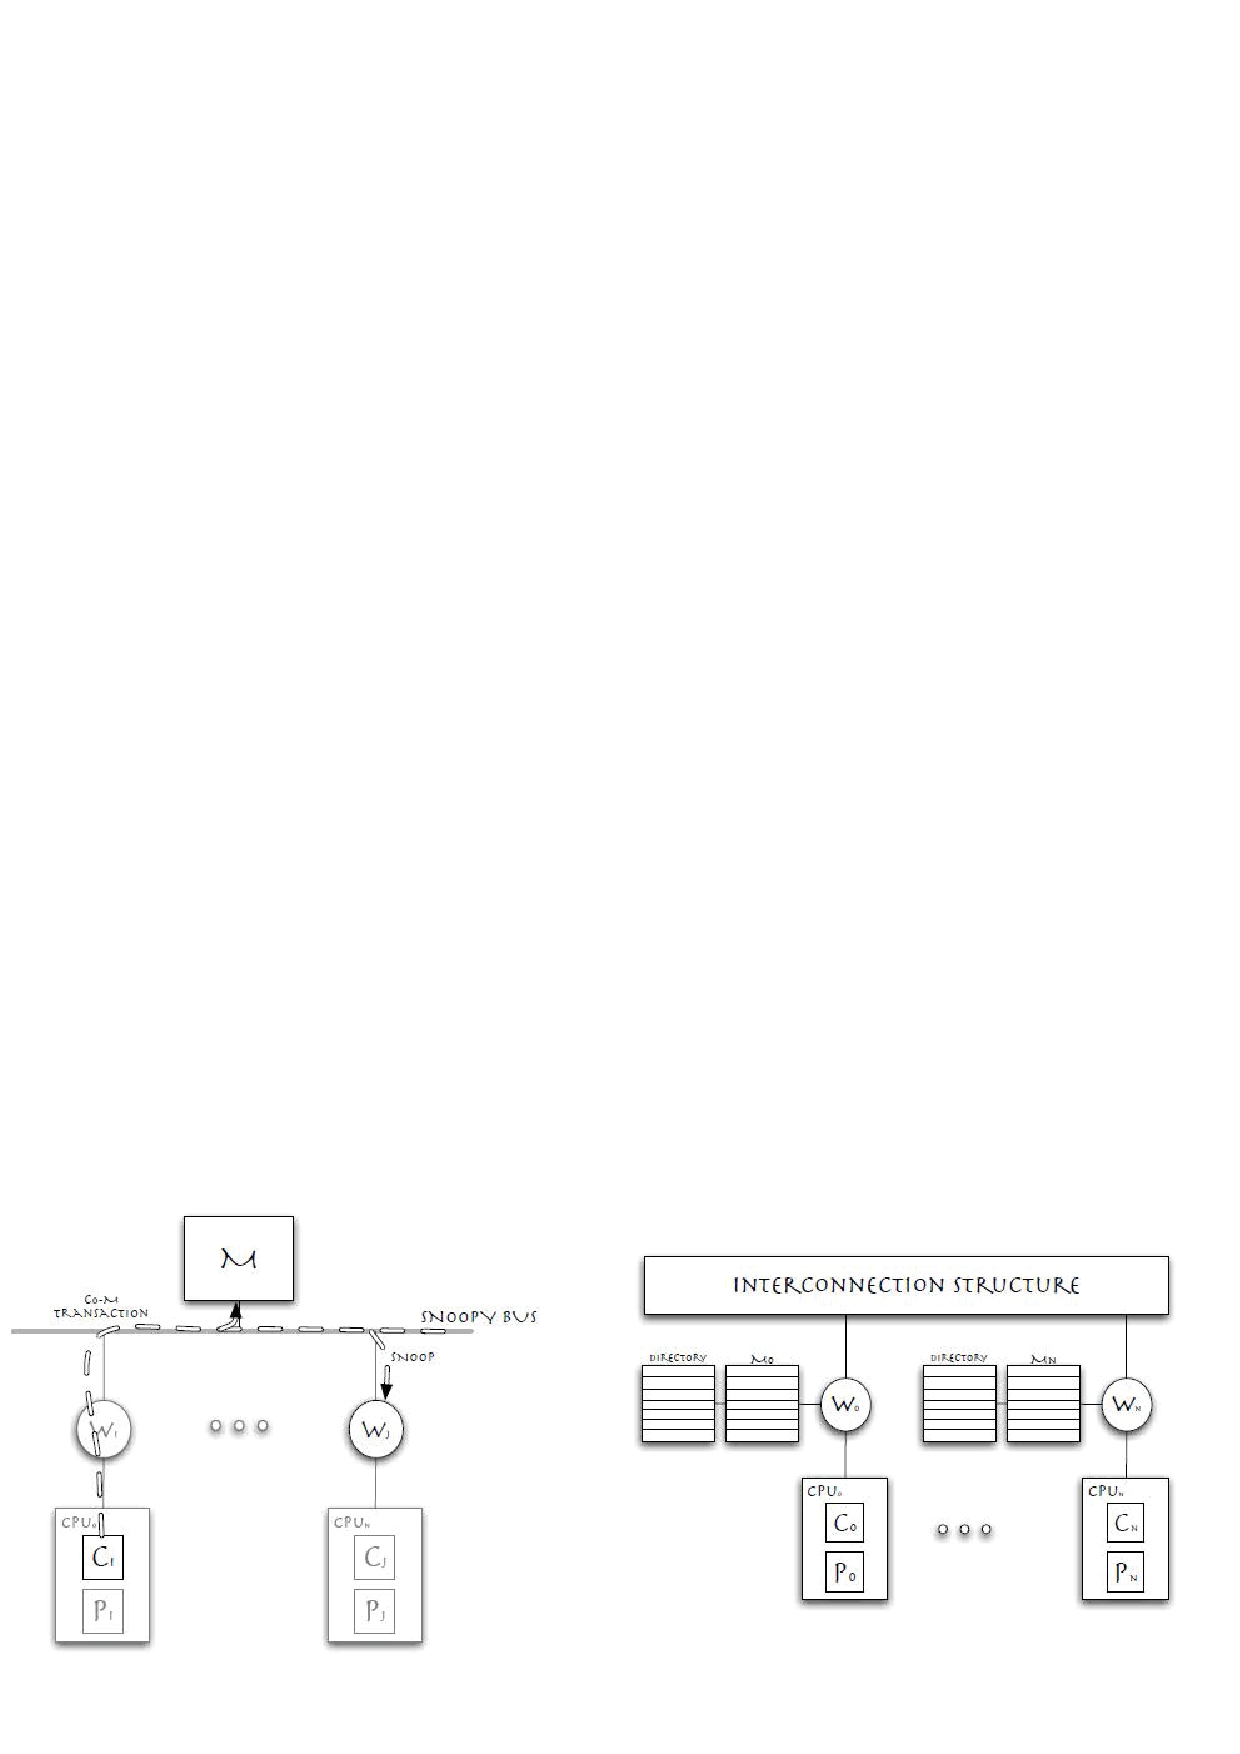
\includegraphics[width=8cm, height=4cm]{./eps/SnoopeDir.png}
 \caption{Snooping and Directory-based protocol}
 \label{fig:s&d}
\end{figurehere}

In all the systems which use the automatic techniques (snooping and directory), a proper protocol must exists in order to perform the required actions atomically. Two main techniques are used: \emph{invalidation}, \emph{update}.\\
Invalidation assumes that the only valid copy of a block is one of those, usually the last one, that has changed, invalidating all other copies (e.g. MSI and MESI in Figure \ref{fig:msimesi}); while update presumes that each modifcation of a cache block copy is communicated (multicasted) to all other caches (e.g. Dragon).\par
\parindent 10mm In the next chapter, invalidation and update techniques will be analysed only on directory-based protocol because it is clear from bibliography that large NUMA system does not support well BUS architecture due to large number of cores and, thus, messages that will limit the bandwith.

\begin{figurehere}
 \centering
 \includegraphics[width=8cm, height=4cm]{./eps/msimesi.png}
 \caption{MESI and MSI protocol}
 \label{fig:msimesi}
\end{figurehere}

%-----------------------------------------------------------------------------
\subsection{Scheduling and memory management \\ Section}

Nowadays 

%%%%%%%%%%%%%%%%%%%%%%%%%%%%%%%%%%%%%%%%%%%%%%%%%%%%%%%%%%%%%%%%%%%%%%%%%%%%%
\section{Evaluation}

In this section it will be discussed the difference between the proposed solutions above giving some value coming from direct confrontation.

%-----------------------------------------------------------------------------
\subsection{Cache coherence \\ Section}

\subsubsection{Cache coherence in NCC-NUMA}
Hardware coherence mechanisms for large-scalemachines are complex and costly, but existing software mechanisms for message-passing machines have not provided a performance-competitive solution. \par 
\parindent 10mm In  [CIT. Multiprocessor cache coherence based on virtual memory support  petersen, Li 1995]  they present a comparative analysis of the performance achived by VM-based algorithm relative to \emph{no caching of shared data} (NO) and the \emph{MESI, invalidation-based, snoopy cache protocol} (Snoop). \\
As it is possible to observe from Figure \ref{fig:result1}, the NO, as expected, it has poor performance for most applications. It is possible to see that there can be a signicant performance gain from using VM-SC, rather than no-caching. However MUL performs best with no caching because only a little over 50% of all shared accesses hit in the cache. \par 
\parindent 10mm The best algorithm VM-based that they proposed is the RC version ( Figure \ref{fig:result1}). In fact the overhead due to coherency faults decreases in VM-RC because of the relaxed memory consistency restrictions, and accounts for most of the improvement of each application. They then compared RC with Snoop; the execution time breakdown for each application shows two reasons for the difference in performance between VM-RC and Snoop: the overhead due to the VM-based implementation of RC, the time a processor stalls on a full write-buffer, and the time a processors spends waiting for memory loads to complete. The cache miss ratio under Snoop and VM-RC is very similar for all applications, therefore the number of memory accesses due to shared and private accesses that require a bus transaction is very close. The total memory access time in VM-RC is affected mostly by memory  accesses issued by the algorithm and due to write-throughs. Relaxing the memory consistency models, and hence synchronizing the processors in the system only  when the application requires to do so, allows the VM-based RC cache coherence scheme to perform very well. 


\begin{figurehere}
 \centering
 \includegraphics[width=6cm, height=3cm]{./eps/Legenda_VM-based.PNG}
 \caption{Legend of next column diagram}
 \label{fig:legend}
\end{figurehere}

\begin{figure*}
 \centering
 \includegraphics[width=14cm, height=7cm]{./eps/result1.PNG}
 \caption{Performance of VM-based schemes}
 \label{fig:result1}
\end{figure*}

\parindent 10mm In their articles,\emph{ Kontothanassis and Scott}[CIT. Software cache coherence for large scale multiprocessores] used virtual memory protection bits to enforce consistency at the granularity of pages allowing more than one processor to write a page concurrently,and used a variant of release consistency to limit coherence operations to synchronization points.\\
As in the work of \emph{Petersen and Li}, they exploit the global physical address space to move data at the granularity of cache lines: instead of copying pages, thay  map them remotely, and allow the hardware to fetch cache lines on demand. The protocol employs a distributed, non-replicated directory data structure that maintains cacheability and sharing information, similar to the coherent map data structure. A page can be in one of the following four states:
\begin{itemize}
    \item \textbf{Uncached}, no processor has a mapping to the page. This
is the initial state for all pages.
    \item \textbf{Shared}, one or more processors have read-only mappings
to the page.
   \item \textbf{Dirty}, a single processor has both read and write mappings
to the page.
   \item \textbf{Weak},  two or more processors have mappings to the page
and at least one has both read and write mappings.
\end{itemize}

\begin{figurehere}
 \centering
 \includegraphics[width=8cm, height=4cm]{./eps/result16proc.png}
 \caption{comparative software and hardware system performance on 16 processors}
 \label{fig:16proc}
\end{figurehere}

They, then, compared their software protocol to the protocol devised by \emph{Petersen and Li}. They found out that their implementation was significantly better then the other and even on applications that in programs where coherence is less important, their protocols still provide reasonable performance improvements over the remaining ones, ranging from 2\% to 35\%.


\begin{figurehere}
 \centering
 \includegraphics[width=8cm, height=4cm]{./eps/result64proc.png}
 \caption{comparative software and hardware system performance on 64 processors}
 \label{fig:64proc}
\end{figurehere}

Int the end, however, they compared their software solutions to hardware existing solutions and find out that in all cases the performance of the software protocol is within 55\% of the hardware protocol as shown in Figure \ref{fig:16proc} and in Figure \ref{fig:64proc}.\par
\parindent 10mm Thus, in the following section will be shown a couple of hardware solutions tipically found on cc-NUMA.

\subsubsection{Cache coherence in CC-NUMA}

As previously said, CC-NUMA have hardware solutions to manage coherency and there exists two different implementation depending on the architecture: BUS or an interconnection structure. According to the implemented architecture, a different solution is used to update and control caches: snooping and directory-based.\par
\parindent 10mm It is important to choose a good protocol for cache coherence on a cache coherent system, thus write invalidate and write update have been examined to choose the best.\par
\parindent 10mm Update protocol conserves bandwidth and needs only one update  transaction to keep multiple sharers up to date but generates a lot of unnecessary traffic when a single processor writes  repeatedly to a block and no other processor accesses the block. On the other hand, invalidate does exactly the opposite and this means that there is not a best solution because both depend on the kind of application running.\par
\parindent 10mm As previously said, there are two hardware architecture: with a bus or with an interconnection structure. Nowadays it is common knowledge that using a bus architecture with a large number of nodes doesn't work very well because this solution presents some problems due to the fact that every request is broadcasted on the BUS and this tends to overfill the bandwidth. Even an interconnection structure has some problems, typically the overhead of directory indirection and message sequencing, but it is a fair price to pay compared to the benefits. [CIT. cache coherent protocols in NUMA multiprocessor - Moh-Hahn, Yoon ]


%-----------------------------------------------------------------------------
\subsection{Scheduling and memory management \\ Section}


% We suggest the use of JabRef for editing your bibliography file (Report.bib)
\bibliographystyle{splncs}
\bibliography{Report}

\end{multicols}
\end{document}
